



\documentclass[12pt]{article}

\usepackage[brazil]{babel}
\usepackage[utf8]{inputenc}
\usepackage{graphicx}
\usepackage{float}
\usepackage{indentfirst}
\usepackage{cite}

\title{Análise da variação do PIB per capita de países asiáticos a partir do desenvolvimento de diferentes industrias}
\author{
	Marcelo Gianfaldoni de Andrade\\
	André Toyama \\
	Lucas Astur \\
}
\date{\today}


\begin{document}
\maketitle

\newpage
\tableofcontents
\newpage

\begin{abstract}
Esse texto busca analisar a variação do PIB per capita de alguns países asiáticos, com foco no Japão, entre os anos 1995 e 2007, baseado em grafos que representam o comportamento de diferentes industrias desse país nesse mesmo intervalo de tempo, com objetivo de entender a relação histórica entre o papel de certas industrias nos países e o desenvolvimento da economia dos mesmos.
\end{abstract}

\section{Introdução}

A partir de um conjunto de dados a respeito do PIB per capita de diversos países do mundo, escolheu-se alguns países que aparentemente apresentavam uma semelhança: uma diminuição no crescimento do PIB per capita por volta do ano de 1997. Esse comportamento pode ser observado na figura \ref{figura1} e na figura \ref{figura2}. A principal hipótese para esse fenômeno é a crise asiática de 1997, detalhada em \cite{crise_asiatica}. Essa hipótese foi feita pela grande semelhança entre a data que os gráficos apresentam a redução do crescimento do PIB per capita e o início da crise citada, e a posição geográfica dos países, os dois asiáticos e detalhados em \cite{crise_asiatica} como grandes afetados por essa crise.

Para uma análise mais profunda, será usado o Japão como exemplo, por ser um país com melhores dados disponibilizados de suas industrias em comparação com a Indonésia. A partir desses dados será feita uma análise de centralidade das industrias no tempo para entender se há alguma relação no comportamento dessas industrias com as alterações no PIB per capita do país, levando em consideração a hipótese de crise em 1997.

\section{Método Utilizado}

Foram utilizadas duas métricas de centralidade para determinar a
importância de cada indústria em seu país: Coreness e PageRank. A partir do
Coreness, é possível determinar quão no centro ou na periferia é a indústria
com relação as outras indústrias do país. A medida do PageRank permite
classificar a centralidade de uma industria analisando o fluxo de riquezas no grafo.

Com a utilização desses dois métodos em conjunto, pode-se fazer uma análise de centralidade mais completa, considerando tanto a posição dele como centro/periferia pelo valor de coreness, quando sua importância no fluxo de riquezas pelo valor de pagerank.

\section{Análise}

Utilizando os métodos de centralidade descritos acima, analisou-se o comportamento das cinco industrias mais centrais do Japão entre 1995 e 2007. O resultado dessa análise pode ser visto na figura \ref{figura3} e na figura \ref{figura4}. Na figura \ref{figura3} pode-se perceber uma grande queda de valor de centralidade na industria com maior valor do país começando desde 1996, e se agravando nos anos seguintes. Essa mesma industria, a com maior valor dentre todas de na figura \ref{figura4}, também sofre uma queda de valor a partir de 1996. 

Observando esse comportamento de uma industria considerada central no Japão, a partir das duas análises de centralidade feitas, pode-se concluir que há evidências que apoiam a relação entre a queda de variação do PIB per capita no país por volta de 1997 e a queda de valor de centralidade da industria considerada mais central na mesma época.

Apenas com essa análise, não é possível concluir se esse é um efeito de causa-consequência, apenas um indicio de uma relação entre a queda de variação do PIB per capita do Japão e a queda de valores de centralidade da industria de Construção no Japão em 1997. Além disso, como explicado anteriormente, é provável que esses dois fenômenos estejam ligados a crise asiática de 1997, que afetou teve o Japão como um dos grandes afetados, como visto em \cite{crise_asiatica}.

\section{Conclusão}

Por fim, encontrou-se evidências o suficiente para entender o fenômeno encontrado visualmente nos gráficos de variação de PIB per capita de diversos países, a mudança brusca em 1997. O fato de todos os países encontrados serem asiáticos aumenta a chance de haver uma relação com a crise asiática de 1997. Além disso, a análise feita no Japão mostra uma possível relação entre esse fenômeno e a queda da industria considerada mais central do país na mesma época, apoiando mais ainda a ideia de uma crise financeira na região.

\section{Anexo}

%---------------------------------------------------------------------------
% Figure
%---------------------------------------------------------------------------
\begin{figure}[H]
	\centering
	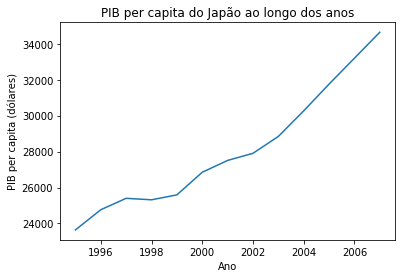
\includegraphics[width=\textwidth]{pib_japao.png}
	\caption{PIB per capita do Japão ao longo dos anos}
	\label{figura1}
\end{figure}

\begin{figure}[H]
	\centering
	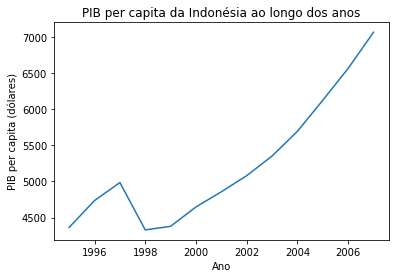
\includegraphics[width=\textwidth]{pib_indo.png}
	\caption{PIB per capita da Indonésia ao longo dos anos}
	\label{figura2}
\end{figure}

\begin{figure}[H]
	\centering
	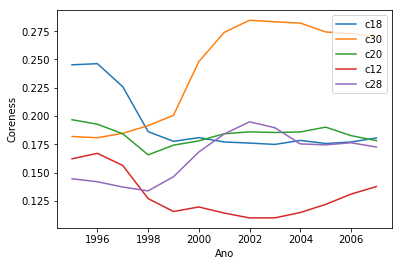
\includegraphics[width=\textwidth]{japan_coreness.png}
	\caption{Coreness das 5 industrias com maiores valores ao longo dos anos}
	\label{figura3}
\end{figure}

\begin{figure}[H]
	\centering
	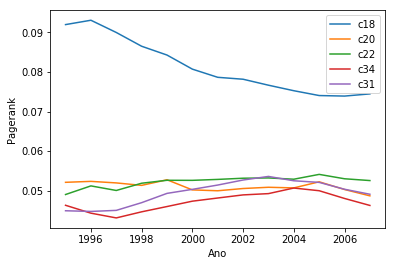
\includegraphics[width=\textwidth]{japan_pagerank.png}
	\caption{Pagerank das 5 industrias com maiores valores ao longo dos anos}
	\label{figura4}
\end{figure}

\begin{figure}[H]
	\centering
	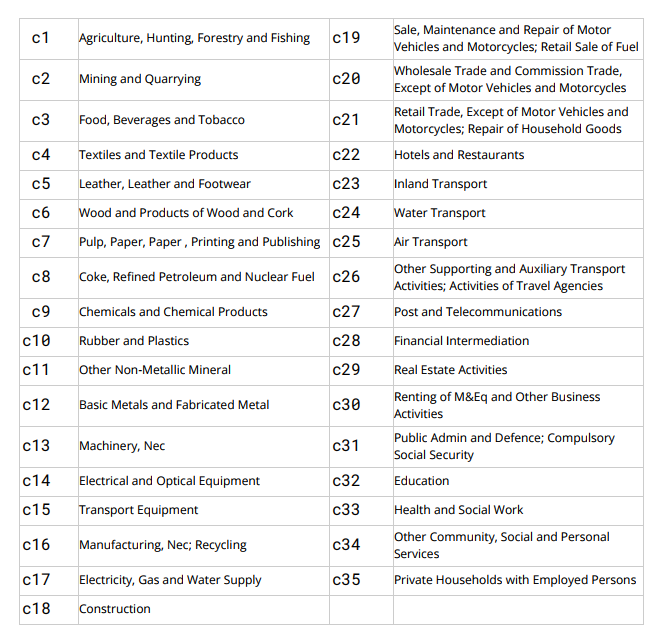
\includegraphics[width=\textwidth]{tabela_industrias.png}
	\caption{Códigos das industrias}
	\label{figura4}
\end{figure}

\bibliography{bibliografia}{}
\bibliographystyle{plain}

%---------------------------------------------------------------------------

\end{document}
  